\chapter{Cryptography techniques}
Cryptography is a mathematical technique that permits to transmit the data to a form that can't be understood by unauthorized users.
\begin{figure}[H]
    \centering
    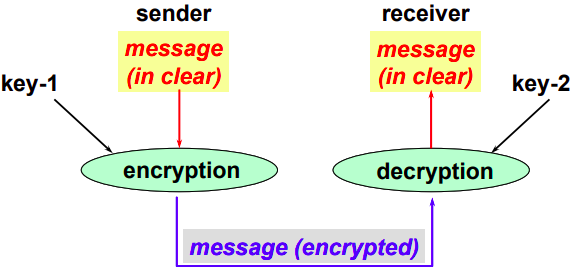
\includegraphics[width=0.5\textwidth]{/home/lorenzo/Notes/Information System Security/images/image copy 13.png}
\end{figure}
\noindent
To explain the various concepts of cryptography we need to introduce some terminology:
\begin{itemize}
    \item \textbf{Plaintext (P)}: the original message before encryption.
    \item \textbf{Ciphertext (C)}: the encrypted message that appears scrambled.
\end{itemize}
\begin{quotebox-grey}{Kerckhoffs' Principle}
\begin{minipage}{0.7\textwidth}
	\vspace{-0.3cm}
This principle states that the security of a cryptographic system should rely on the \textbf{secrecy of the keys}, not the secrecy of the encryption algorithm itself. 
If the keys:
\begin{itemize}
\item are kept secure, this ensures only authorized parties can decrypt the message.
\item are managed by trusted systems, this minimizes the risk of unauthorized access.
\item are of adequate length, they are harder to crack with brute force methods. 
\end{itemize} 
\end{minipage} 
\hspace{0.3cm}
\begin{minipage}{0.3\textwidth}
    \centering
    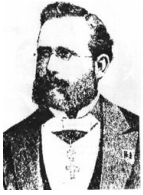
\includegraphics[width=0.4\textwidth]{/home/lorenzo/Notes/Information System Security/images/image copy 14.png}
\end{minipage}
\noindent
\\
\\
\textbf{It's no important that the encryption and decryption algorithms are kept secret}, on the contrary it's better to make the algorithms public so that they can be widely analysed and their possible weakness identified. 
\\
\\
Kerchoff’s Principle is tightly correlated to the principle of \textbf{Security Through Obscurity
(STO)}: a system is protected but the details on how it has been protected are not disclosed.
This alone is not considered a valid security mechanism. STO can be used as a layer of the security system \textbf{only if} a really strong algorithm is used
\end{quotebox-grey}
\newpage
\section{Symmetric Cryptography}
\textbf{Symmetric cryptography} is so called because it uses \textbf{only} a single key \textbf{shared between} the sender and the receiver. 
\[key1=key2=K\]
The key \textbf{K} is used to generate the Ciphertext \textbf{C} by encrypting the Plaintext \textbf{P}. \textbf{C} is then sent to the receiver, which recovers \textbf{P} by applying the decryption algorithm using \textbf{K}:
\[C\ =\ enc(K,P)\ =\ \{P\}K\]
\[P\ =\ dec(K,C)\ =\ enc^{-1}(K,C)\]
\begin{figure}[H]
    \centering
    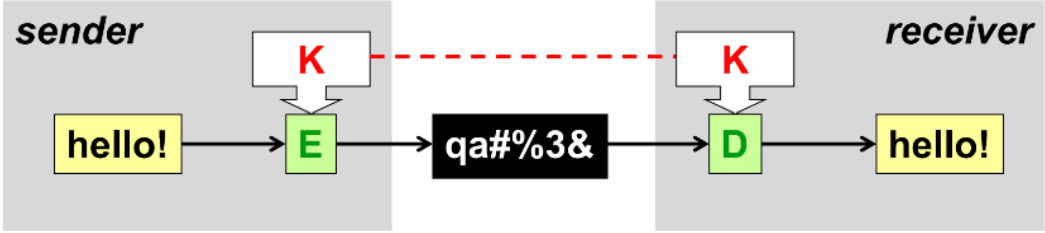
\includegraphics[width=0.5\textwidth]{/home/lorenzo/Notes/Information System Security/images/Screenshot from 2024-12-27 13-04-27.png}
\end{figure}
\noindent
\textbf{Symmetric Encryption} requires the use of a unique \textbf{K} for each peer couple. A complete pairwise private communication between N parties would requires \(\frac{N \cdot (N-1)}{2}\) unique \textbf{K}s.\\
The parties can exchanged \textbf{securely} the \textbf{K}s in two ways:
\begin{itemize}
    \item \textbf{OOB} (\textbf{Out-Of-Band}): the parties share the \textbf{K} without using electronic channel used for transmitting the encrypted message.
    \item \textbf{Exchange algorithms}: looks bellow at \textbf{Asymmetric Encryption Algorithms}.
\end{itemize}